\subsection{单态射的锥；连接同态的新定义}

现在考虑复形的一个正合列

\[
0 \rightarrow \mathrm{C} ^ {\prime} \xrightarrow {u} \mathrm{C} \xrightarrow {v} \mathrm{C} ^ {\prime \prime} \rightarrow 0.\tag{9}
\]

定义一个次数为0的分次A-线性映射

\[
\varphi : \operatorname{Con} (u) \rightarrow \mathrm{C} ^ {\prime \prime}
\]

由 \(\varphi(y', x) = v(x)\) 定义。于是我们有一个行正合的 A-模交换图

\[
\begin{array}{c} 0 \longrightarrow \mathrm{C} ^ {\prime} \stackrel {{\tilde {u}}} {{\longrightarrow}} \mathrm{Cyl} (u) \stackrel {{\tilde {\pi}}} {{\longrightarrow}} \mathrm{Con} (u) \longrightarrow 0 \\ 1 \Big \downarrow \qquad \qquad \qquad \beta \Big \downarrow \qquad \qquad \qquad \varphi \Big \downarrow \\ 0. \longrightarrow \mathrm{C} ^ {\prime} \stackrel {{u}} {{\longrightarrow}} \mathrm{C} \stackrel {{v}} {{\longrightarrow}} \mathrm{C} ^ {\prime \prime} \longrightarrow 0. \end{array}\tag{10}
\]

命题9. --- 映射 β 和 φ 是复形的拟同构。对于 β ，这由命题7，c）得出。我们有

\[
\begin{array}{r l} \varphi \circ \mathrm{D} (y ^ {\prime}, x) & = \varphi (- d ^ {\prime} y ^ {\prime}, d x - u (y ^ {\prime})) = v (d x - u (y ^ {\prime})) \\ & = v (d x) = d ^ {\prime \prime} v (x) = d ^ {\prime \prime} (\varphi (y ^ {\prime}, x)), \end{array}
\]

因此 \(\varphi\) 确实是一个复形态射。另一方面， \(\varphi\) 是满射的，且其核被等同于复形 \((\mathbf{K}, d_{\mathbf{K}})\) ，其中 \(\mathbf{K} = \mathbf{C}'(-1) \oplus \mathbf{C}'\) ,

\[
d _ {\mathbf {K}} (y ^ {\prime}, x ^ {\prime}) = (- d ^ {\prime} y ^ {\prime}, d ^ {\prime} x ^ {\prime} - y ^ {\prime});
\]

如果 \(d_{\mathbf{K}}(y', x') = 0\) ，则 \(y' = d'x'\) ，从而 \((y', x') = d_{\mathbf{K}}(0, -x')\) ；由此可知 \(\mathrm{H}(\mathbf{K}) = 0\) ，且 \(\varphi\) 是拟同构（X，第 30 页，推论 1）。

注记。--- 拟同构 β 是同伦等价，但 φ 一般不是同伦等价（参见 X，第 173 页，习题 8）。

推论。——分次A-模的图表

\pandocbounded{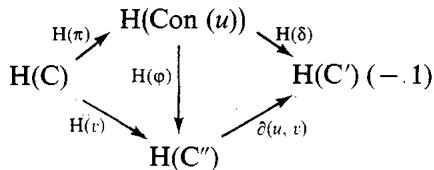
\includegraphics[keepaspectratio]{images/part001_82ee8f27.jpg}}

是可交换的，且H(φ)是双射。

在交换图（10）中，我们有 \(\mathrm{H}(1_{\mathbf{C}^{\prime}})\circ \partial (\tilde{u},\tilde{\pi}) = \partial (u,v)\circ \mathrm{H}(\varphi)\) （X，第31页，命题2）和 \(\partial (\tilde{u},\tilde{\pi}) = \mathrm{H}(\delta)\) （X，第38页，引理3，b）），因此

\[
\partial (u, v) \circ \mathbf {H} (\varphi) = \mathbf {H} (\delta);
\]

另一方面， \(\mathrm{H}(v) \circ \mathrm{H}(\beta) = \mathrm{H}(\varphi) \circ \mathrm{H}(\tilde{\pi}) = \mathrm{H}(\varphi) \circ \mathrm{H}(\pi) \circ \mathrm{H}(\beta)\) 根据X，第39页，注记。由于 \(\mathrm{H}(\beta)\) 是双射的，这给出 \(\mathrm{H}(v) = \mathrm{H}(\varphi) \circ \mathrm{H}(\pi)\) .

我们因此有 \(\partial(u, v) = H(\delta) \circ H(\varphi)^{-1}\) ，它为连接同态 \(\partial(u, v)\) 提供了一个新的定义。我们还注意到，如果把 \(H(Con(u))\) 与 \(H(C'')\) 借助 \(H(\varphi)\) 等同起来，则前面的推论表明，正合列（8）此时等同于相对于（9）的同调正合列。

